\section{Objectives}
By the end of this laboratory assignment, students are expected to learn how to 

\begin{itemize}

\item use C libraries for interfacing general-purpose input-output (GPIO) pins with a single-board computer and   
  
\item implement a simple traffic light control algorithm using onboard LEDs of a single-board computer.  
 
  
\end{itemize}

\section{Parts}
\label{sec:partsTLC}
The following parts are required to conduct this laboratory assignment. %
%
\begin{enumerate}
\item BBBlue board with the latest OS (debian) image installed
\item One micro-USB cable  
\end{enumerate}

\section{Background}
\label{sec:background}

This laboratory assignment is primarily meant to use some C library functions of the robotics cape package, \emph{librobotcontrol}, for controlling onboard LEDs and GPIO pins on the BBBlue single-board computer (SBC). The \emph{librobotcontrol} package is pre-installed in the BBBlue board. In this laboratory assignment, we shall focus on implementing  algorithms that emulate the following applications:
%
\begin{enumerate}
    \item Flashing red light and 
    \item Traffic light controller at an intersection of two one-way roads.
\end{enumerate}
%

Before implementing the algorithms that emulate the above applications, it is important to review the working principles of these applications.

\subsection{LEDs}
\label{sec:LEDs}
The BBBlue board has eleven LEDs that are accessed using the following application programming interfaces (APIs).
\begin{center}
\begin{verbatim}
RC_LED_GREEN
RC_LED_RED
RC_LED_USR0
RC_LED_USR1
RC_LED_USR2
RC_LED_USR3
RC_LED_BAT25
RC_LED_BAT50
RC_LED_BAT75
RC_LED_BAT100
RC_LED_WIFI
\end{verbatim}
\end{center}
%
Each LED on the BBBlue board is labeled so that it is easily identfied with the API name mentioned above. These LEDs are controlled using the following functions (from \emph{rc/led.h}):
\begin{verbatim}
  rc_led_set (rc_led_t led, int value)
  rc_led_cleanup (void)
\end{verbatim}
The \emph{rc\_led\_set} function is used to turn an LED on or off. To call this function, the name of the LED to control is passed as the \emph{led} argument, and the desired state is passed as the \emph{value} (0 for off, nonzero for on). For example, the following statement would turn on the onboard green LED:
\begin{verbatim}
  rc_led_set (RC_LED_GREEN, 1);
\end{verbatim}
To properly close out the LEDs before exiting the program, the \emph{rc\_led\_cleanup} function should be called at the end of the program.

\subsection{GPIO Pins}
\label{sec:GPIOPins}
The BBBlue board has several GPIO pins that can be used to receive inputs or drive outputs. The pins accessible on ports GP0 and GP1 are shown in \autoref{fig:GPIO_pins}. These pins can be connected to external hardware (pushbuttons, LEDs, etc) to provide added functionality to the board.
%
\begin{figure}
  \centering
  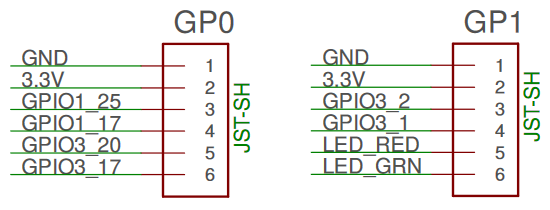
\includegraphics[width= 0.5\textwidth]{figs/img/Lab1/GPIO_pins.png}
  \caption{BBBlue GPIO Ports 0 and 1}
  \label{fig:GPIO_pins}
\end{figure}
%
The GPIO pins are controlled using the following functions (from \emph{rc/gpio.h}):
\begin{verbatim}
  rc_gpio_init (int chip, int pin, int handle_flags)
  rc_gpio_get_value (int chip, int pin)
  rc_gpio_set_value (int chip, int pin, int value)
  rc_gpio_cleanup (int chip, int pin)
\end{verbatim}
Each of these functions requires inputs of both a chip and a pin. In \autoref{fig:GPIO_pins}, the GPIO pins are labeled as \emph{GPIOx\_y}, where \emph{x} is the chip number, and \emph{y} is the pin number. For example, pin 4 of GP1 is on pin 1 of chip 3. When the pin is initialized, it must be configured as either an input or an output by passing either \emph{GPIOHANDLE\_REQUEST\_INPUT} or \emph{GPIOHANDLE\_REQUEST\_OUTPUT} for the \emph{handle\_flags} parameter of \emph{rc\_gpio\_init}. For example, the following statement would be used to set pin 4 of GP1 as an output:
\begin{verbatim}
  rc_gpio_init (3, 1, GPIOHANDLE_REQUEST_OUTPUT);
\end{verbatim}
The value of a pin configured as an input can be obtained as the return value of the \emph{rc\_gpio\_get\_value} function. To set the output value of a pin configured as an output, the \emph{rc\_gpio\_set\_value} function is used. If a zero is passed as the value, the GPIO pin is set to off (inactive), while a nonzero value turns the pin on (active). To properly close out the GPIO pin before exiting, the \emph{rc\_gpio\_cleanup} function should be called at the end of the program on each GPIO pin that was used.

NOTE: The LED\_RED and LED\_GRN pins of GP1 are connected to the onboard red and green LEDs, and thus are controlled using the LED functions rather than the GPIO functions. See \autoref{sec:LEDs} for details on using the LEDs.

\subsection{Flashing Red Light}
\label{sec:FlashingRedLight}
A flashing red light turns on and off at a certain frequency. It is normally used at an  intersection of roads where traffic comes to a complete stop. A circuit that emulates a flashing red light is shown in \autoref{fig:flashingLED1}.  A square wave voltage $v_s(t)$ for $t\ge 0$ mimics ON-OFF signals provided by the SBC. 
%
\begin{figure}
    \centering
    \begin{circuitikz}[scale=1.2,american voltages]
      \draw (0,0) to[sqV,v<=$v_s(t)$ (binary input from SBC),fill=green!50]
      (0,4*\smgrid) to[R,v>=$R$](5*\smgrid,4*\smgrid) to[full led,o-o,l^=~~~LED
      (Red),v>=~](5*\smgrid,0) to[short,-*] (0,0) node[ground]{};
    \end{circuitikz}
    \caption{Circuit for emulating a flashing light.}
    \label{fig:flashingLED1}
\end{figure}
%
Therefore, the input is a binary voltage that is to be sent to turn on and off of an LED using an algorithm to be implemented on BBBlue. The LED can be chosen from one of the onboard LEDs. Note that resistor is not needed to be connected if an onbard LED is used. If an external LED is used, a GPIO pin must be used to drive the LED.

\subsection{Traffic Light Controller}
\label{sec:voltageDivider}
In this part, a simple traffic light control logic is to be implemented on a SBC. For simplicity, we will be considering traffic lights at the intersection of two one-way roads: East-West (EW) and North-South (NS) as shown in \autoref{fig:intersection1}. Three LEDs are used to indicate the traffic signals for each road: one Green, one Yellow, and  one Red. At any given time, there is an \emph{active direction} with its lights set to green  and an \emph{inactive direction} with its lights set to red. In the active direction, the duration of Green, Yellow, and Red lights are $10~[\second]$ (state\#1), $4~[\second]$ (state\#2) and $2~[\second]$ (state\#3), respectively.  The duration of Red light in the inactive direction is $16~[\second].$ The active and inactive directions are then switched. A full light cycle passes through three states as described in \autoref{tab:traffic1}, where logic $1(0)$ represent that the corresponding LED  is ON (OFF). %
%
\begin{figure}
  \centering
  \begin{tikzpicture}[scale=0.6]
    % East-West
    \draw[very thick]
    (-5,1) -- (5,1)node[anchor=west]{\textcolor{ForestGreen}{$\bullet$~\textbf{Green}}};
    \draw
    (5,0) node[anchor=west]{\textcolor{YellowOrange}{$\bullet$~\textbf{Yellow}}};
    \draw[very thick,red,dashed]
    (-5,-1) -- (5,-1)node[anchor=west]{\textcolor{BrickRed}{$\bullet$~\textbf{Red}}};
    \draw[ultra thick,->]
    (-5,0)node[anchor=east]{East} --(-3,0);
    \draw
    (8,0) node[anchor=west]{West};

    % North-South
    \draw[very thick]
    (-1,5) -- (-1,-5)node[anchor=south,rotate=90]{\textcolor{ForestGreen}{$\bullet$~\textbf{Green}}};
    \draw
    (0.5,-5) node[anchor=south,rotate=90]{\textcolor{YellowOrange}{$\bullet$~\textbf{Yellow}}};    
    \draw[very thick,red,dashed]
    (1,5) -- (1,-5)node[anchor=north,rotate=90]{\textcolor{BrickRed}{$\bullet$~\textbf{Red}}};
    \draw[ultra thick,->]
    (0,5)node[anchor=south]{North} --(0,3);
    \draw
    (0,-8) node[anchor=north]{South};
  \end{tikzpicture}
  \caption{Traffic lights at an intersection of two one-way roads.}
  \label{fig:intersection1}
\end{figure}

\begin{table}%[htbp]
\caption{Traffic light cycle.}
\label{tab:traffic1}
\centering
\begin{tabular}{c|c|c|c}
\toprule
Direction & State~\#1 ($10~[\second]$) & State~\#2 ($4~[\second]$) & State~\#3 ($2~[\second]$)\\
\toprule
Active (\textcolor{ForestGreen}{Green}, \textcolor{YellowOrange}{Yellow}, \textcolor{BrickRed}{Red}) & (1, 0, 0) & (0, 1, 0) & (0,0,1)\\
\hline
Inactive (\textcolor{ForestGreen}{Green}, \textcolor{YellowOrange}{Yellow},\textcolor{BrickRed}{Red}) & (0, 0, 1) & (0, 0, 1) & (0, 0, 1)\\
\bottomrule
\end{tabular}

\end{table}


\begin{prelab}[Flashing RED light]{prelab:flashingRedLight}
  Suppose that the LED, RC\_LED\_RED, of the BBBlue board is used  to mimic a flashing Red light at an intersection of roads. You are to write a C program in a BBBlue board so that it practically flashes the LED at the frequency of $0.5~[\hertz].$ The program should perform the  following operations.
  \begin{enumerate}
  \item When PAU button is pressed, the LED practically flashes at the frequency of $0.5~[\hertz].$
  \item When MOD button is pressed, the LED stops flashing (LED is OFF) and the program terminates.      
  \end{enumerate}
\end{prelab}




\section{Laboratory Work}

You are to write a C program in a BBBlue board so that it practically implements a traffic light control logic at an intersection of  two one-way roads. Use the onboard LEDs of the BBBlue to configure the traffic lights as illustrated in \autoref{tab:tlc2}. %
%
\begin{table}
  \centering
  \caption{LED configurations for implementing traffic light controller. }
  \label{tab:tlc2}  
  \begin{tabular}{l|l}
    \toprule   
    East--West & North--South\\
    \toprule
    RC\_LED\_GREEN $\to$ Green & RC\_LED\_USR1 $\to$ Green\\   	    
    RC\_LED\_USR0 $\to$ Yellow  	  & RC\_LED\_USR2 $\to$ Yellow\\  
    RC\_LED\_RED 	$\to$ Red          & RC\_LED\_USR3 $\to$ Red\\  
    \bottomrule    
  \end{tabular}
\end{table}
%
State durations of traffic lights are given in  \autoref{tab:traffic1}. The program should perform the  following operations.


\begin{enumerate}
\item When PAU button is pressed, the LEDs in active and inactive directions
  will flash as per the state durations given in \autoref{tab:traffic1}.
\item When MOD button is pressed, all LEDs are OFF and the program terminates.
\end{enumerate}
 

%%% Local Variables:
%%% mode: latex
%%% TeX-master: "../../labBookMechatronics-V2"
%%% End:
